
\vspace{-5pt}
\section{\relbench Datasets}
\vspace{-5pt}
\label{sec:datasets}

\begin{wrapfigure}[11]{r}{0.55\textwidth}
    \vspace{-25pt} % Adjust this value as needed to reduce or increase space above the figure
    \centering
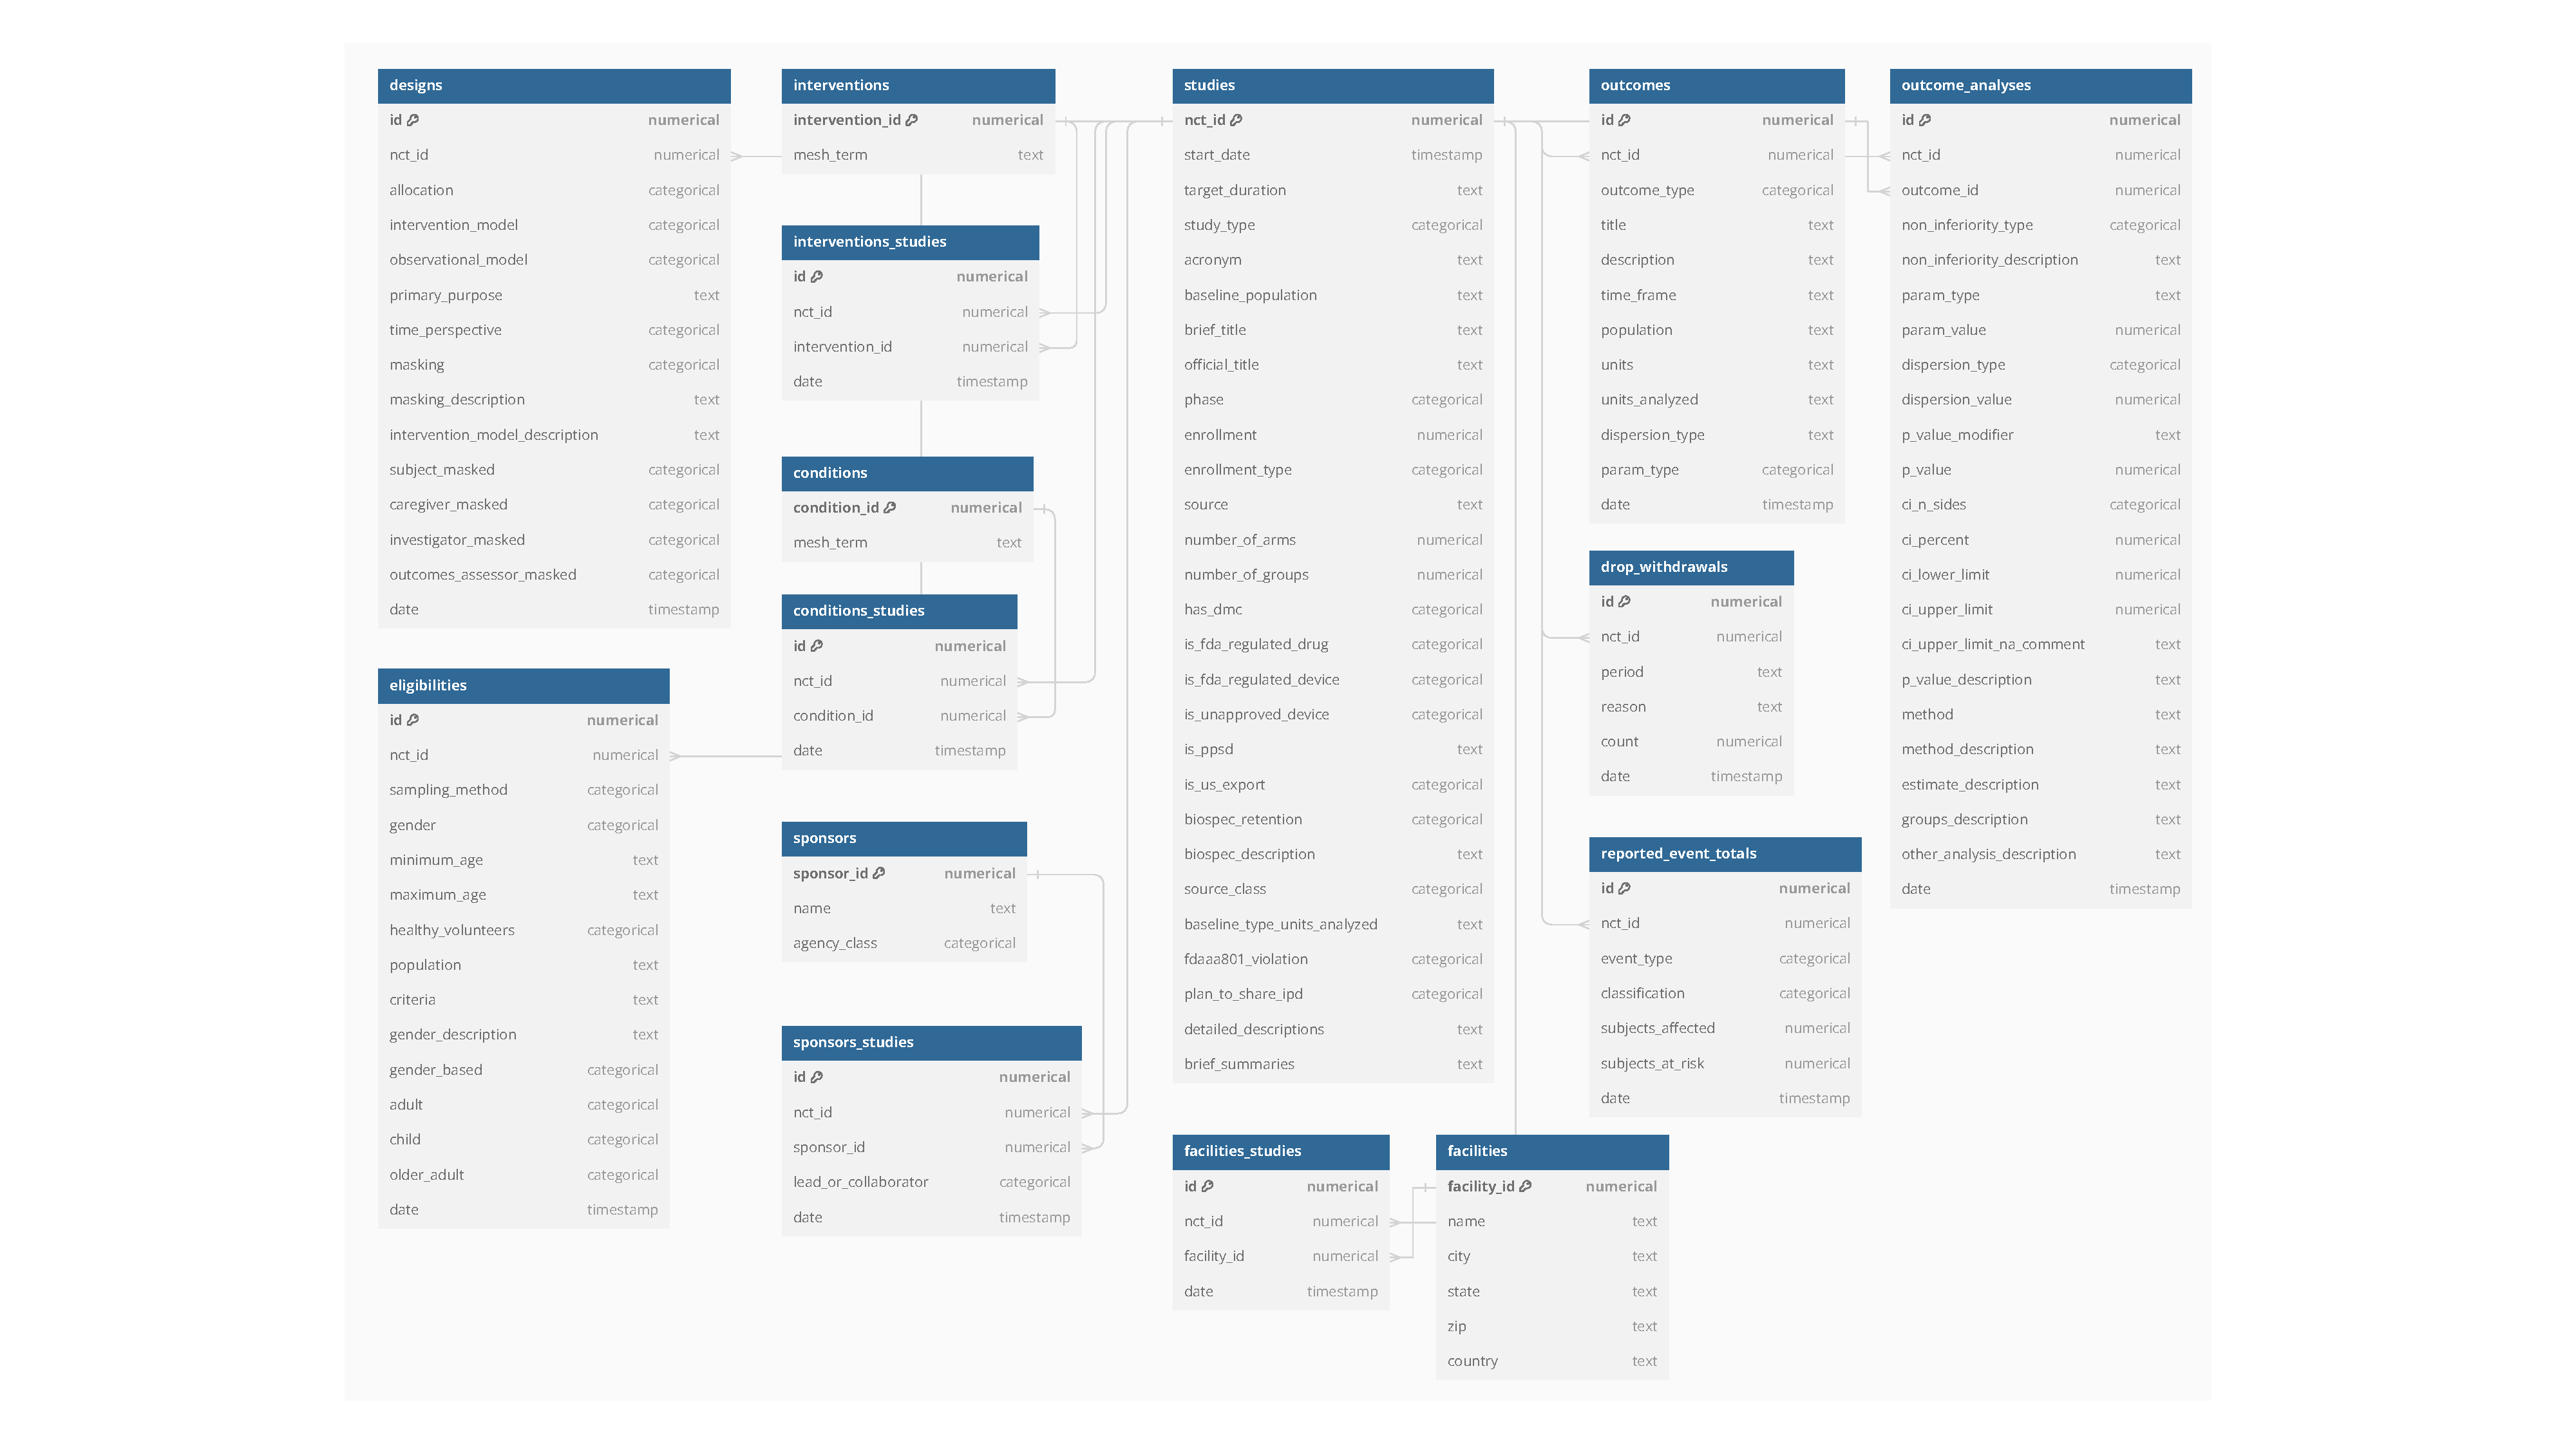
\includegraphics[width=0.4\textwidth]{figs/trial.pdf}
    \vspace{-10pt} % Adjust this value as needed to reduce or increase space between the figure and the caption
    \caption{Example \relbench schema for \trials. \relbench databases have complex relational structure and rich column features. }
    \vspace{+20pt}
    \label{fig:dbdiagram}
\end{wrapfigure}



\relbench contains 7 datasets each with rich relational structure, providing a challenging environment for developing and comparing relational deep learning methods (see Figure \ref{fig:dbdiagram} for an example). The datasets are carefully processed from real-world relational databases and span diverse domains and sizes. 
Each database is associated with multiple individual predictive tasks defined in Section~\ref{sec:tasks}. 
Detailed statistics of each dataset can be found in Table~\ref{tab:datasets_stats}. We briefly describe each dataset.

\xhdr{\amazon} The Amazon E-commerce database records products, users, and reviews across Amazon's E-commerce platform. It contains rich information about products and reviews. Products include the price and category of each, reviews have the overall rating, whether the user has actually bought the product, and the text of the review itself. We use the subset of book-related products.

\xhdr{\fone} The F1 database tracks all-time Formula 1 racing data and statistics since 1950. It provides detailed information for various stakeholders including drivers, constructors, engine manufacturers, and tyre manufacturers. Highlights include data on all circuits (\eg 
 geographical details), and full historical data from every season. This includes overall standings, race results, and more specific data like practice sessions, qualifying positions, sprints, and pit stops. 

\xhdr{\stackex} Stack Exchange is a network of question-and-answer websites on different topics, where questions, answers, and users are subject to a reputation award process. The reputation system allows the sites to be self-moderating. The database includes detailed records of activity including user biographies, posts and comments (with raw text), edit histories, voting, and related posts.  In our benchmark, we use the stats-exchange site. 

\begin{table}[t]
  \centering
  \caption{{Full list of predictive tasks for each \relbench dataset (introduced in Table~\ref{tab:datasets_stats}).}  }
  \label{tab:task_stats}
  \renewcommand{\arraystretch}{1.1}
  \setlength{\tabcolsep}{4pt}
  % \resizebox{\linewidth}{!}{
  \tiny
  \begin{tabular}{lllccclll}
    \toprule
      \mr{2}{\textbf{Dataset}} & \mr{2}{\textbf{Task name}} & \mr{2}{\textbf{Task type}} & \mc{3}{c}{\textbf{\#Rows of training table}} & \#Unique & \%train/test & \#Dst \\
      & & & Train & Validation & Test & Entities & Entity Overlap  & Entities \\
    \midrule
      \mr{6}{\amazon}
      & \userChurn & entity-cls & 4,732,555 & 409,792 & 351,885 & 1,585,983 & 88.0 & --- \\
      & \itemChurn & entity-cls & 2,559,264 & 177,689 & 166,842 & 416,352 & 93.1 & ---  \\
      & \userLtv & entity-reg  & 4,732,555 & 409,792 & 351,885 & 1,585,983 & 88.0 & --- \\
      & \itemLtv & entity-reg   & 2,707,679 & 166,978 & 178,334 & 427,537 & 93.5 & ---\\
      & \userItemPurchase & recommendation   & 5,112,803 & 351,876 & 393,985 & 1,632,909 & 87.4 & 12,562,384\\
      & \userItemRate & recommendation  & 3,667,157 & 257,939 & 292,609 & 1,481,360 & 81.0 & 7,665,611\\
      & \userItemReview & recommendation  & 2,324,177 & 116,970 & 127,021 & 894,136 & 74.1 & 5,406,835\\
    \midrule
    \mr{4}{\avito}
    & \adsCTR & entity-reg & 5,100 & 1,766 & 1,816 & 4,997 & 59.8 &---\\
    & \userClick & entity-cls & 59,454 & 21,183 & 47,996 & 66,449 & 45.3 &---\\
    & \userVisit & entity-cls & 86,619 & 29,979 & 36,129 & 63,405 & 64.6 &---\\
    & \userAdVisit & recommendation & 86,616 & 29,979 & 36,129 & 63,402 & 64.6 & 3,616,174\\
    \midrule
    \mr{3}{\event}
    & \userAttendance & entity-reg & 19,261 & 2,014 & 2,006 &9,694 & 14.6&---\\
    & \userRepeat & entity-cls & 3,842 & 268 & 246 &1,514 & 11.5&---\\
    & \userIgnore & entity-cls & 19,239 & 4,185 & 4,010 &9,799 & 21.1&---\\
    \midrule
    \mr{3}{\fone}
      & \driverDNF & entity-cls & 11,411 & 566 & 702 & 821 & 50.0 & --- \\
      & \driverTopThree & entity-cls  & 1,353 & 588 & 726 & 134 & 50.0 & --- \\
      & \driverPosition & entity-reg & 7,453 & 499 & 760 & 826 & 44.6 & --- \\
      % & \driverConstructorResult & recommendation & 893 & 73 & 57 & 728 & 5.3 & 2,147 \\
    \midrule
    \mr{3}{\handm}
      & \userChurn & entity-cls  & 3,871,410 & 76,556 & 74,575 & 1,002,984 & 89.7 & --- \\
      & \itemSales & entity-reg & 5,488,184 & 105,542 & 105,542 & 105,542 & 100.0 & --- \\
      & \userItemPurchase & recommendation & 3,878,451 & 74,575 & 67,144 & 1,004,046 & 89.2 & 13,428,473 \\
    \midrule
    \mr{5}{\stackex}
      & \userEngage & entity-cls & 1,360,850 & 85,838 & 88,137 & 88,137 & 97.4 & --- \\
      & \userBadge & entity-cls  & 3,386,276 & 247,398 & 255,360 & 255,360 & 96.9 & --- \\
      & \postVotes & entity-reg  & 2,453,921 & 156,216 & 160,903 & 160,903 & 97.1 & --- \\
      & \userPostComment & recommendation  & 21,239 & 825 & 758 & 11,453 & 59.9 & 44,940 \\
      & \postPostLinked & recommendation  & 5,855 & 226 & 258 & 5,924 & 8.5 & 7,456 \\
    \midrule
    \mr{5}{\trials}
      & \studyOutcome & entity-cls  & 11,994 & 960 & 825 & 13,779 & 0.0 & --- \\
      & \studyAdverse & entity-reg  & 43,335 & 3,596 & 3,098 & 50,029 & 0.0 & --- \\
      & \facilitySuccess & entity-reg  & 151,407 & 19,740 & 22,617 & 129,542 & 42.0 & --- \\
      & \sponsorConditionRec & recommendation  & 36,934 & 2,081 & 2,057 & 3,956 & 98.4 & 533,624 \\
      & \sponsorFacilityRec & recommendation  & 669,310 & 37,003 & 27,428 & 445,513 & 48.3 & 1,565,463 \\
   \bottomrule
  \end{tabular}
  % }
\end{table}

\xhdr{\trials} The clinical trial database is curated from AACT initiative, which consolidates all protocol and results data from studies registered on ClinicalTrials.gov. It offers extensive information about clinical trials, including study designs, participant demographics, intervention details, and outcomes. It is an important resource for health research, policy making, and therapeutic development.

\xhdr{\handm} The H\&M relational database hosts extensive customer and product data for online shopping experiences across its extensive network of brands and stores.  This database includes detailed customer purchase histories and a rich set of metadata, encompassing everything from basic demographic information to extensive details about each product available. 

\xhdr{\event} The Event Recommendation database is obtained from user data on a mobile app called Hangtime. This app allows users to keep track of their friends' social plans. The database contains data on user actions, event metadata, and demographic information, as well as users' social relations, which captures how social relations can affect user behavior. Data is fully anonymized, with no personally identifiable information (such as names or aliases) available.

\xhdr{\avito} Avito is a leading online advertisement platform, providing a marketplace for users to buy and sell a wide variety of products and services, including real estate, vehicles, jobs, and goods. The Avito Context Ad Clicks dataset on Kaggle is part of a competition aimed at predicting whether an ad will be clicked based on contextual information. This dataset includes user searches, ad attributes, and other related data to help build predictive models.


\xhdr{Data Provenance} All data is sourced from publicly available repositories with licenses permitting usage for research purposes. See Appendix \ref{app:data} for details of data sources, licenses, and more.  


